\chapter*{Preface}
\addcontentsline{toc}{chapter}{Preface}

The Tape server project is targeted at replacing the CAStor tape server with a new drop-{}in reimplementation. The reimplementation will replace a legacy implementation that is written in C.

The reimplementation will be done using the latest tools available to us in the current Scientific Linux distribution. The language will be C++, to group concept and variables in self-contained
(and unit testable) objects.

The interface to the mounting deamons might still change with repect to CAStor 2.1.14 as the mounting daemons are being reviewed in parallel.

This documentation itself currently references the older tape server this project is intending to replace. The references will have to be removed as they become unnecessary. 
Likewise, the layout of the document will be adapted.

The tape drive primitives have now been developed, and the rest of the project's
plan is being laid out.

% ------------------------------------------------------------------------------ 
% Chapter: Developer's manual
% ------------------------------------------------------------------------------

\chapter{Developer's manual}

% Section:  Requirements
% ------------------------------------------------------------------------------
\section{Requirements}

\subsection{Targeted environment}

CERN SLC5 and SLC6, 64bits. Although it should compile in theory, the 32 bits version is not tested. The unit test purposely returns an error when run on non-64 bits architecture.

\subsection{Pre-existing requirements}

The new tape server (software) will have to replace the software running on a tape server
(computer). A previous analysis describes the current software stack of the tape servers
	\footnote{ \href{http://svn.cern.ch/guest/CASTOR/CASTOR2/trunk/castor/tape/doc/TapeBridge.pdf}
	{http://svn.cern.ch/guest/CASTOR/CASTOR2/trunk/castor/tape/doc/TapeBridge.pdf}}.
This new tape server will retain the same external interfaces as the old tape server, replacing 
the stack of daemons from the tape bridge down to the tape drive hardware.

The tape server will interface with the Volume and Drive Queue Manager daemon (vdqmd), the Volume
manager daemon (vmgrd), the Castor User Privilege Validation daemon (cupvd) and tape gateway 
daemon (tapegatewayd) for data transfer management and access control.

It will connect to the CAStor disk servers to transfer the data itself, using one of the supported
protocols (current candidates are rfio, xroot and ceph) and it will use the services of the Remote 
Media Changer daemon (rmcd) to mount and unmount tapes.

\subsubsection{Tape session triggering}

The tape server acts as a server only on one occasion, when it receives a client info request from the 
VDQM. This call triggers a tape session, recall or migrate. The information received at that point
is only client system information and drive information (request ID, host, port, DGN, tape drive name and user information (user id, etc...)).

The main thread of the tape server will then just forks (and maybe exec, to be decided (TODO)) a new
process, which will handle the session and quit.

A new session starts with the tape server connecting with the client (it could be the tape gateway, or one of the command line commands of castor (currently packages in castor-tapebridge-client: readtp, writetp, 
dumptp). In the case of the tape gateway, it can be either a read or a write session.

The collaboration diagrams of the previous version of the tape server (with all its sub components)
can be found in dot format
	\footnote{ \href{http://svn.cern.ch/guest/CASTOR/CASTOR2/trunk/castor/tape/doc/collaboration\_diagrams/}
	{http://svn.cern.ch/guest/CASTOR/CASTOR2/trunk/castor/tape/doc/collaboration\_diagrams/}}.
	
The new sequencing of a session start, simplified from the internal component communication is shown here:

\begin{center}
\begin{sequencediagram}
	\newthread{vm}{vmgrd}
	\newthread{vd}{vdqmd}
	\newthread{ts}{tapeserverd(main)}
	\newinst{tsc}{tapeserverd(child)}
	\newthread{gw}{client(gateway or command line)}
	
	\begin{call}{gw}{get volume}{vm}{tape VID}
	\end{call}
	\begin{call}{gw}{vdqm request/volume stuff}{vd}{VDQM request ID}
	\end{call}
	\begin{call}{vd}{schedule}{vd}{}
	\end{call}
	\begin{call}{ts}{unitStatus(UP)}{vd}{}
	\end{call}
	\begin{call}{vd}{schedule}{vd}{}
	\end{call}
	\begin{call}{vd}{VDQM\_CLIENTINFO}{ts}{}
	\end{call}
	\begin{call}{ts}{fork}{tsc}{}
		\begin{call}{tsc}{Volume request}{gw}{}
		\end{call}
		\begin{call}{tsc}{Proceed with session}{tsc}{}
		\end{call}
	\end{call}

\end{sequencediagram}
\end{center}

At that point, already two client libraries are in use in the tape server: the {\bf{}tape gateway protocol client} library and the {\bf{}vdqm client} library, and a simple server, answering only one type or requests:

\begin{itemize}
\item{}The client library for the tape gateway is implemented using the UML/umbrello based serialisation system. It is contained in the \verb#castor::tape::tapebridge::ClientProxy# class in CAStor.
\item{}The direct C client API in CAStor's \verb#h/vdqm_api.h#.
\item{}The VDQM request handler is implemented in the server class \verb#castor::tape::tapebridge::VdqmRequestHandler#.
\end{itemize}

\subsubsection{Tape session startup}

Upon reception of the session request, the tape server checks that it can continue with the session:
\begin{itemize}
\item{}with VMGR the volume status and block size. A disabled volume can only be mounted by a TP\_OPER (this information is retrieved from cupv).
\item{}In case of a write session, it queries the pool info know the owner. If user is not the owner or ADMIN, refuse the mount.
\end{itemize}

Then reports are sent:
\begin{itemize}
\item{}Reports to VDQM that the drive is assigned. (VDQM\_UNITSTATUS).
\item{}Requests work to be done from the client to prevent useless mounts (and start caching data 
in case of migration.
\item{}Mounts the tape, rewinds and validates the volume label.
\item{}Reports to VMGR that the volume is mounted (\verb#VMGR_TPMOUNTED#).
\item{}Reports to the VDQM that the tape is mounted (VDQM\_UNITSTATUS).
\end{itemize}

This part adds the {\bf{}vmgr client} and the {\bf{}rmcd client}.

TODO: bad day scenario.

\subsubsection{Work loop}
The work loop will be a 4 step pipelined operation where:
\begin{itemize}
\item{}The work to be done FIFO gets topped up continuously  by a thread (using bulk)
\item{}The data FIFO(s) is(are) filled up by the reader (tape thread or disk thread).
\item{}The data FIFO consumer (opposite)
\item{}The results are reported by either the control thread or a specialized thread (using bulk).
\end{itemize}

\subsubsection{Release tape}

\subsection{Extra requirements}
Additional requirements, arising from the current practices of operators are:

\begin{itemize}
\item{}The tape server's session should gracefully handle an unclean situation where the 
tape is left in the drive by a previously crashed session. The protocol is to clean anything
left over before proceeding to the new session.
\item{}A tape sessions should be preemptable by the operator. This is currently achieved 
by killing the tape process. Closing the session on a kill (-1) could be a solution.
\item{}The operator should be able to specify values in different SCSI code pages in
order to setup the tape drive. This setting will be defined differently for each tape
drive type.
\end{itemize}

\section{Tape server architecture}
To fulfil the requirement for an ability to kill a session, the main tape server daemon
will be simple, and just report its status to the VDQM and wait for requests from it on
an open port.

When a tape mount should start, the process will fork a child process, which will reserve the memory
and instantiate the tape mount machinery.

The layout of the main process is show in figure \ref{tsParentProcess}. The layout of the child process, which contains all the complexity is shown in figure \ref{tsChildProcess}.

\begin{figure}[h]
\begin{center}
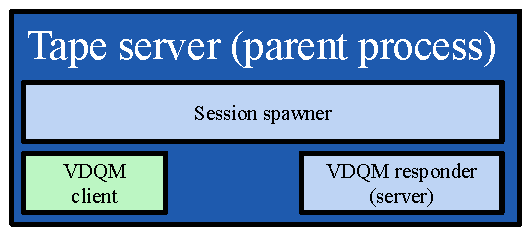
\includegraphics{images/TapeServerParentProcess}
\end{center}
\caption{\label{tsParentProcess}Tape server parent process: libraries used (purpose built libraries in blue, system libraries in beige, already existing CAStor libraries in green)}
\end{figure}


\begin{figure}[h]
\begin{center}
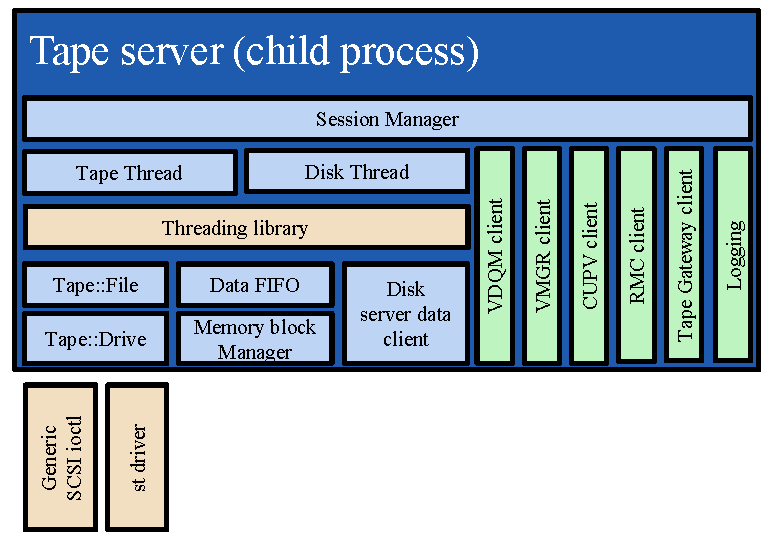
\includegraphics{images/TapeServerChildProcess}
\end{center}
\caption{\label{tsChildProcess}Tape server child process: libraries used (purpose built libraries in blue, system libraries in beige, already existing CAStor libraries in green)}
\end{figure}

The data path will go to/from tape drive, through the generic SCSI interface of st driver (CAStor uses a
mixture of both in the Tape::Drive class), then through the File structure support class, as controlled by
the tape thread. The tape thread will communicate the data to (or get from) the disk threads via the 
data FIFO class. This class will in turn allocate the memory from a preallocated, pool of
fixed sized blocks. The size of the pool will be controlled by the operators.

Some libraries already exist in CAStor, and will be reused, either by copying or linking from pre-compiled 
packages. The main parts of the sessions spawner will be taken from the VDQM as well.

\subsubsection{Memory management and threading architecture}
Like the previous version in rtcpd, the tape server will pre-allocate a fixed number of memory
blocks for the whole duration of the tape session, and circulate them between the data producers 
and consumers.

The data flow is organised around block passing, from queue to queue. Each queue output is processed
by a thread of thread pool.

The overall layout of a migration mount is shown in figure \ref{tsMigrationMM}. The recall mount, shown in\
figure \ref{tsRecallMM}, is almost symmetric. The report packer triggers on threshold instead of tape 
flushes, and 

\begin{figure}[h]
\begin{center}
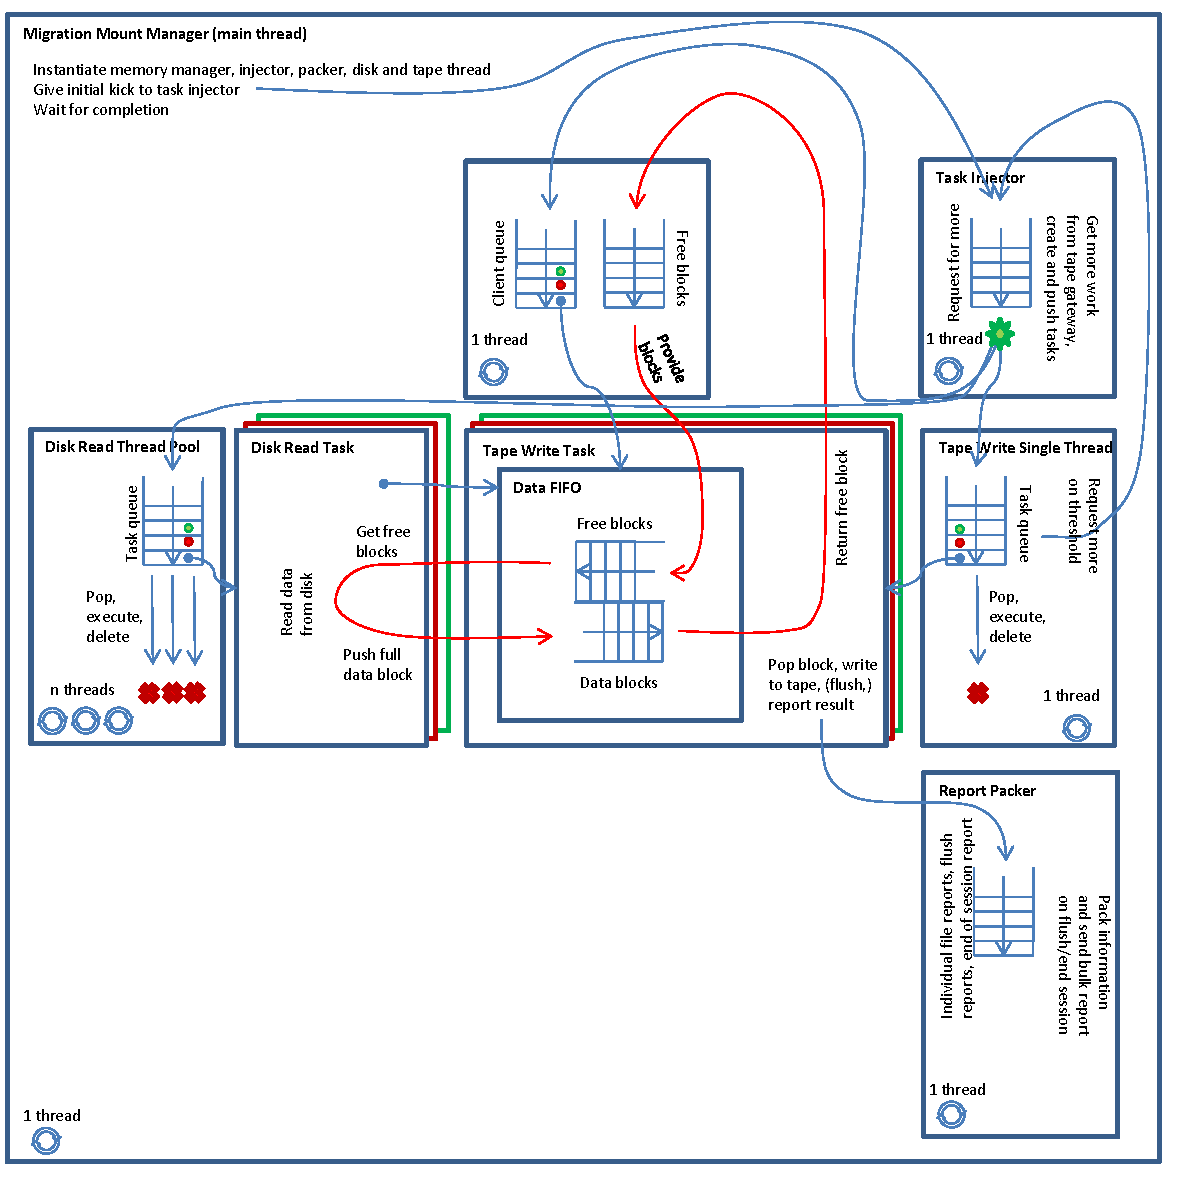
\includegraphics[scale=0.75]{images/MigrationMountMM}
\end{center}
\caption{\label{tsMigrationMM}Tape server child process: layout of the memory management in the case
of a migration mount}
\end{figure}

\begin{figure}[h]
\begin{center}
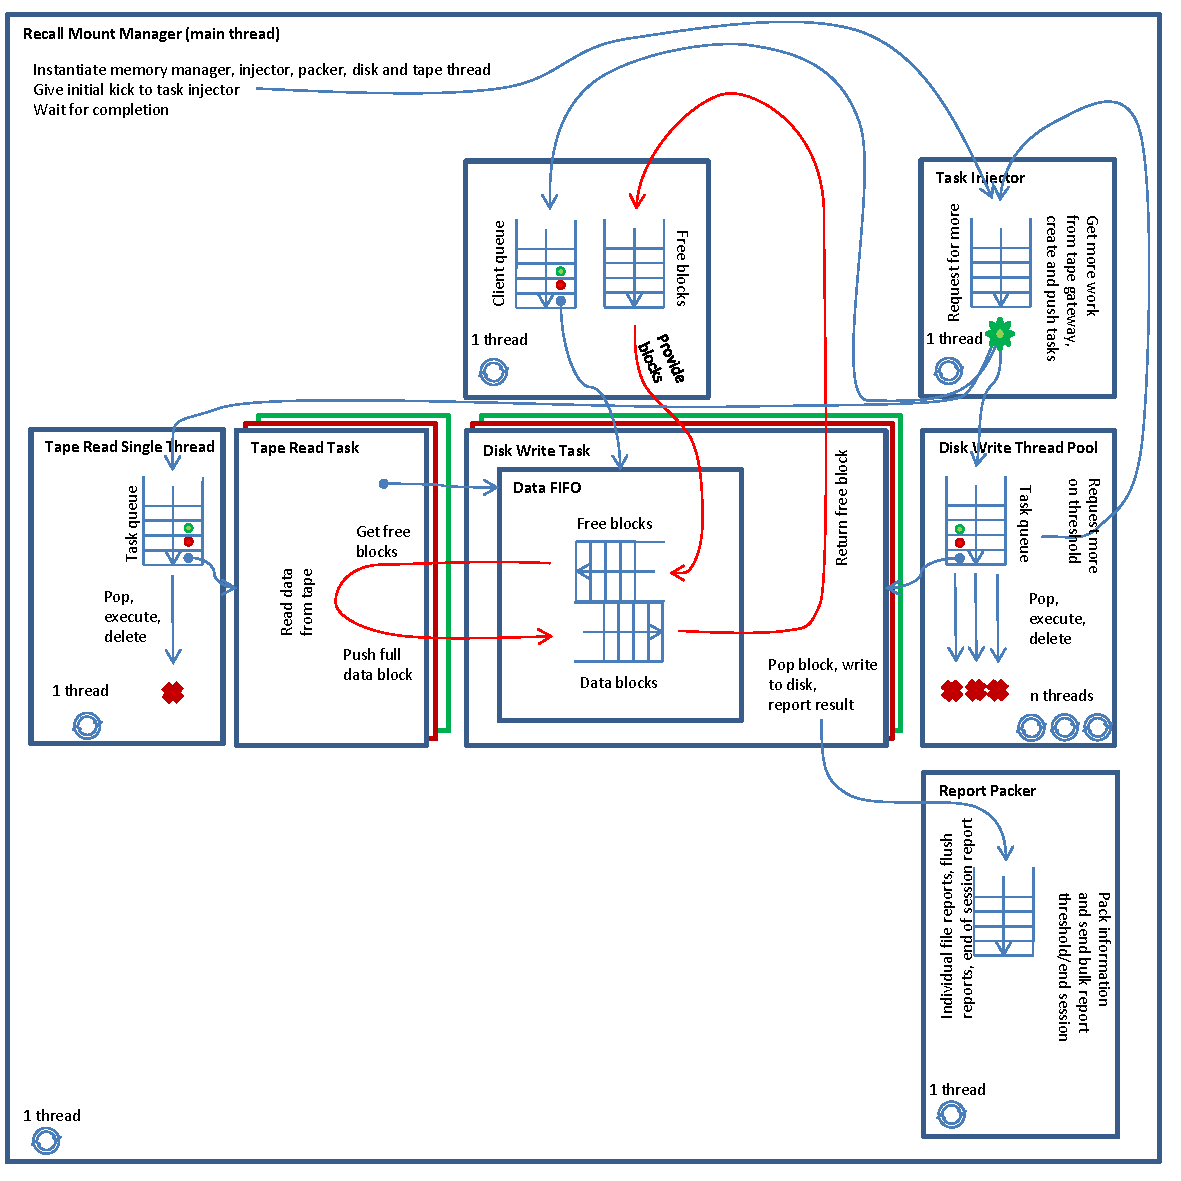
\includegraphics[scale=0.75]{images/RecallMountMM}
\end{center}
\caption{\label{tsRecallMM}Tape server child process: layout of the memory management in the case
of a recall mount}
\end{figure}


% Section:  Reference documentations
% ------------------------------------------------------------------------------

\section{Reference documentations}
\subsection{SCSI specifications}

The SCSI commands can be found in the SCSI section of Hackipedia.org
      \footnote{ \href{http://hackipedia.org/Hardware/SCSI/}{http://hackipedia.org/Hardware/SCSI/} }
      \footnote{The official site for SCSI standard is \href{http://T10.org}{http://T10.org}. All specifications
      can be found there in their approved version, but behind a paywall. Nevertheless all previous drafts were
      public and can conveniently be found on the web. Hackipedia hold a very nice collection of such
      documentations.}.
 The most significant documents for tape server development are the SCSI stream commands (SSC-3
      \footnote{ \href{http://hackipedia.org/Hardware/SCSI/Stream\%20Commands/SCSI\%20Stream\%20Commands\%20-\%203.pdf}
                      {http://hackipedia.org/Hardware/SCSI/Stream\%20Commands/SCSI\%20Stream\%20Commands\%20-\%203.pdf} })
 and the SCSI primary commands (SPC-4
      \footnote{ \href{http://hackipedia.org/Hardware/SCSI/Primary\%20Commands/SCSI\%20Primary\%20Commands\%20-\%204.pdf}
                      {http://hackipedia.org/Hardware/SCSI/Primary\%20Commands/SCSI\%20Primary\%20Commands\%20-\%204.pdf} }).

\subsubsection{Manufacturer's specificities}
\label{Manufacturer's specificities}
The SCSI specification allows for some flexibility for the manufacturers of tape drives, and 
each of them has differences. The details can be found in the following documentations:

\begin{itemize}
\item{}StorageTek\texttrademark T10000 Tape Drive
       \footnote{ \href{http://docs.oracle.com/cd/E19957-01/96174E/96174E.pdf}
                       {http://docs.oracle.com/cd/E19957-01/96174E/96174E.pdf} }
\item{}Sun StorageTek\texttrademark T10000 Tape Drive Fibre Channel Interface Reference Manual
       \footnote{ \href{http://docs.oracle.com/cd/E19772-01/MT9259L/MT9259L.pdf}
                       {http://docs.oracle.com/cd/E19772-01/MT9259L/MT9259L.pdf} }
\item{}IBM System Storage TS1120 and TS1130 Tape Drives and TS1120 ControllerOperator Guide3592 Models J1A, E05, E06, EU6, J70 and C06
       \footnote{ \href{ftp://ftp.software.ibm.com/storage/TS1130/a86opg02.pdf}
                       {ftp://ftp.software.ibm.com/storage/TS1130/a86opg02.pdf} }
\item{}IBM System Storage Tape Drive 3592 SCSI Reference
       \footnote{ \href{http://www-01.ibm.com/support/docview.wss?uid=ssg1S7003248\&aid=1}
                       {http://www-01.ibm.com/support/docview.wss?uid=ssg1S7003248\&aid=1} }
\item{}IBM TotalStorage LTO Ultrium Tape Drive SCSI Reference  (LTO-5 through LTO-6)
       \footnote{ \href{http://www-01.ibm.com/support/docview.wss?uid=ssg1S7003556\&aid=1}
                       {http://www-01.ibm.com/support/docview.wss?uid=ssg1S7003556\&aid=1} }
\end{itemize}

\subsection{SCSI support in Linux}
On the Linux side, the main references are the Linux 2.4 SCSI subsystem HOWTO
       \footnote{ \href{http://mirrors.kernel.org/LDP/HOWTO/pdf/SCSI-2.4-HOWTO.pdf}
                       {http://mirrors.kernel.org/LDP/HOWTO/pdf/SCSI-2.4-HOWTO.pdf} },
especially for its section 9.3 on the st driver,
and the Linux SCSI Generic (sg) HOWTO 
       \footnote{ \href{http://mirrors.kernel.org/LDP/HOWTO/pdf/SCSI-Generic-HOWTO.pdf}
                       {http://mirrors.kernel.org/LDP/HOWTO/pdf/SCSI-Generic-HOWTO.pdf} }. 

More details regarding the Generic SCSI driver can be found on the SCSI subsystem maintainer's web site 
       \footnote{ \href{http://sg.danny.cz/sg/}{http://sg.danny.cz/sg/} }.

The section on the SG\_IO ioctl, \footnote{ \href{http://sg.danny.cz/sg/sg\textunderscore{}io.html}{http://sg.danny.cz/sg/sg\textunderscore{}io.html} } details the usage of the 
simplest ioctl for the generic SCSI driver, which allows the invocation of a SCSI command and the collection of the 
result in a single system call.

This ioctl is provided in the middle layer of the SCSI subsystem of Linux. All SCSI drivers, st included, fall back
to the middle layer when encountering an unknown ioctl. This means there is no need to open the matching generic SCSI,
unless we want to control command queueing with separate sending of commands and result collection, which
requires the use of read and write calls from the generic SCSI (sg) driver.

\subsection{Unsorted CAStor docs}
A collection of links to various documentations written in the past is available on one of CAStor's web pages
       \footnote{ \href{http://castorwww.web.cern.ch/castorwww/links.htm}{http://castorwww.web.cern.ch/castorwww/links.htm} }.

\subsection{SCSI tape support in Linux (st driver)}
Generic SCSI allows detailed control of the operations, but the bulk of them (including reading and
writing) can be managed by the higher level SCSI tape (or st) driver provided by the Linux kernel.
More information on the st driver can be found in the man page "st" and in \verb#Documentation/scsi/st.txt#
in the sources of the kernel.

\section{Tools used during development}
\subsection{Required tools for build}
\begin{itemize}
\item{}GCC/G++ (Basic SLC version)
\item{}CMake (Basic SLC version)
\item{}rpmbuild (Basic SLC version)
\item{}Google Mock/Google test (GTest is provided in EPEL repository for SLC. 
  GMock requires recompilation. The source RPMs can be found for newer versions of RPM based distributions, for example from rpmfind 
  \footnote{ \href{http://rpmfind.net/linux/rpm2html/search.php?query=gmock}{http://rpmfind.net/linux/rpm2html/search.php?query=gmock} }.
 For convenience, 
  they are also available on AFS as a temporary solution
      \footnote{ \href{file:///afs/cern.ch/user/c/canoc3/public/GoogleTest-Mock}{/afs/cern.ch/user/c/canoc3/public/GoogleTest-Mock} }.
\item{}Valgrind (Basic SLC version)
\item{}\LaTeX (Basic SLC version) to compile this document
\item{}Doxygen for code documentation (Basic SLC version)
\end{itemize}

\subsection{Tools used during development}
\begin{itemize}
\item{}mhvtl \footnote{ \href{https://sites.google.com/site/linuxvtl2/}{https://sites.google.com/site/linuxvtl2/} } for developing against virtual drives and libraries (to enable mhvtl kernel debug output to dmesg opts=3 have to be used for kernel module options, i.e.
\small{}\verb#modprobe mhvtl opts=3# ).
\item{}TeamCity for continuous integration
\item{}NetBeans as an IDE, including for remote development\
\end{itemize}

\subsection{Code coverage using lcov}
Although the code coverage is not integrated in the build process, it is
straightforward to run on the code. The following recipe will deliver a set of 
web pages indicating which parts of the code are covered or not in the unit tests.
The lcov package is required. It is only available on SLC6, and can be installed via yum.
\begin{itemize}
\item{}Change the main CMakeFiles.txt as in this diff:
\begin{small}
\begin{verbatim}
Index: CMakeLists.txt
===================================================================
--- CMakeLists.txt      (revision 76)
+++ CMakeLists.txt      (working copy)
@@ -45,7 +45,8 @@
 ###########################################################################
 # compiler options
 ###########################################################################
-set (CMAKE_CXX_FLAGS "-g3 -Wall -Werror -pedantic -O2")
+set (CMAKE_CXX_FLAGS "-g3 -Wall -Werror -pedantic -O2 --coverage")
+set (CMAKE_LD_FLAGS "--coverage")

 ###########################################################################
 # dependancies
\end{verbatim}
\end{small}

\item{}Re-run cmake, recompile as usual and run the unit test.
\item{}Capture the result:

        \small{}\verb#lcov --capture --directory 00build/ --output-file 00build/coverage.info#.
\item{}\normalsize{}Generate the resulting html pages: 
        
        \small{}\verb#genhtml 00build/coverage.info --output-directory 00build/coverage#.
\end{itemize}

\section{Software layout}

\subsection{SCSI structures, constants and endianness}

In order to make the code readable, and to avoid heavy mask-and-shift usage (which one would tend
to code using litterals in order to avoid many constants definitions), we use bit field structures.
The unused fields can be left anonymous.
The definition is shown in listing \ref{SCSI_struct}, and usage in listing \ref{SCSI_struct_usage}.
As there could be endianness issues, we limit this usage to within bytes. Fortunately, the SCSI 
standard nicely adheres to this rule.

\begin{table}[h]
\begin{lstlisting}[caption=SCSI::Structures example,label=SCSI_struct]
namespace SCSI {
  namespace Structures {

    /*
     * Inquiry data as described in SPC-4.
     */
    typedef struct {
      unsigned char perifDevType : 5;
      unsigned char perifQualifyer : 3;

      unsigned char : 7;
      unsigned char RMB : 1;

      unsigned char version : 8;

      unsigned char respDataFmt : 4;
      unsigned char HiSup : 1;
      unsigned char normACA : 1;
      unsigned char : 2;
[...]
    } inquiryData_t;
  }
}
\end{lstlisting}
\end{table}

\begin{table}[h]
\begin{lstlisting}[caption=SCSI::Structures usage example,label=SCSI_struct_usage]
      SCSI::Structures::inquiryData_t & inq = *((SCSI::Structures::inquiryData_t *) dataBuff);
      std::stringstream inqDump;
      inqDump << std::hex << std::showbase << std::nouppercase
              << "inq.perifDevType=" << (int) inq.perifDevType << std::endl
              << "inq.perifQualifyer=" << (int) inq.perifQualifyer << std::endl
[...]
              << "inq.T10Vendor="      << SCSI::Structures::toString(inq.T10Vendor) << std::endl
              << "inq.prodId="         << SCSI::Structures::toString(inq.prodId) << std::endl
              << "inq.prodRevLv="      << SCSI::Structures::toString(inq.prodRevLvl) << std::endl
              << "inq.vendorSpecific1="<< SCSI::Structures::toString(inq.vendorSpecific1)<< std::endl
\end{lstlisting}
\end{table}

The unit test resorts to shift and mask, once and only once, to validate the bit fields in
another way. There is an example for this validation in \verb#SCSI/StructureTest.cc# an excerpt is in listing \ref{SCSI_struct_testing}.

\begin{table}
\begin{lstlisting}[caption=SCSI::Structures usage example,label=SCSI_struct_testing]
namespace UnitTests {
  TEST(SCSI_Structures, inquiryData_t_multi_byte_numbers_strings) {
    /* Validate the bit field behavior of the struct inquiryData_t,
     which represents the standard INQUIRY data format as defined in 
     SPC-4. This test also validates the handling of multi-bytes numbers,
     as SCSI structures are big endian (and main development target is 
     little endian.  */
    unsigned char inqBuff [100];
    memset(inqBuff, 0, sizeof(inqBuff));
    SCSI::Structures::inquiryData_t & inq = *((SCSI::Structures::inquiryData_t *) inqBuff);
    /* Peripheral device type */
    ASSERT_EQ(0, inq.perifDevType);
    inqBuff[0] |= (0x1A & 0x1F) << 0;
    ASSERT_EQ(0x1A, inq.perifDevType);
    
    /* Peripheral qualifier */
    ASSERT_EQ(0, inq.perifQualifyer);
    inqBuff[0] |= (0x5 & 0x7) << 5;
    ASSERT_EQ(0x5, inq.perifQualifyer);
[...]
  }
}
\end{lstlisting}
\end{table}

Other common types in the SCSI specification are multi-bytes
number, which are represented by \verb#unsigned char[2/* (or 4)*/]# and handled by helper functions 
\verb#toU16()# and \verb#toU32()#. The helper functions
conveniently use \verb#ntoh{l|s}#, as SCSI and network orders are the same. The reverse
is covered by \verb#setU16()# and \verb#setU32()#. Another helper function 
takes care of string extraction from fixed sized char arrays. See listing \ref{SCSI_data_helpers}.

\begin{table}
\begin{lstlisting}[caption=SCSI::Structures helper functions,label=SCSI_data_helpers]
SCSI::Structures::uint32_t toU32(const char(& t)[4]);
SCSI::Structures::uint32_t toU32(const char(& t)[4]);

template <size_t n>
std::string toString(const char(& t)[n]);
\end{lstlisting}
\end{table}

Those arrays are space-padded, and may not be 0 terminated. It is seen in listing \ref{SCSI_struct_usage}.
The helper function extracts the string, dealing with potential zeros at the end,
and the fixed length. They keep the space-padding at the end of the extracted
string.

To avoid literals in the code, which forces anyone reading it to do tedious lookups,
the SCSI constants are also defined as constants in the code. See listing \ref{SCSI_consts}.

\begin{table}
\begin{lstlisting}[caption=SCSI::Constants,label=SCSI_consts]
namespace SCSI {
  class Commands {
  public:
    enum {
      /*
       *      SCSI opcodes, taken from linux kernel sources
       *      Linux kernel's is more complete than system's
       *      includes.
       */
      TEST_UNIT_READY                               = 0x00,
      REZERO_UNIT                                   = 0x01,
      REQUEST_SENSE                                 = 0x03,
[...]
\end{lstlisting}
\end{table}

Finally all structures have a constructor, which at least zeroes all the data.
Some structures (typically the CDBs, where the first byte is the operation's code)
automatically set the value of fields which can only have one value. Helper
functions are created as needed, where accessing/setting the data in the structure
requires non-trivial processing (and when the case is not covered by the common
tools handling strings that endianness).

\subsection{Exceptions hierarchy and error handling strategy}

There is a small class hierarchy for exceptions: \verb#Tape::Exception# inherits from
\verb#std::exception#, and \verb#Tape::Exceptions::Errnum# inherits from the latter.
\verb#Tape::Exceptions::Errnum# manages the errnos. It collects the errno value and turns it
into a string automatically at construction time.

\verb#Tape::Exception# and all its heirs automatically generate a stack trace at creation time.
This allows easy tracing of unhandled exceptions, as the stack trace is embedded in the content
of the \verb#what()# method. For the cases where the exception is indeed handled, a shorter version
called \verb#shortWhat()# allows the logging of the problem without bloating the logs with long stack 
traces.

Another exception class, \verb#SCSI::Exception#, turns the SCSI status and sense buffer into a
user readable string. In addition, a helper exception thrower function avoids code
repetitions (\verb#ExceptionLauncher()#).

Throughout the project, the error handling strategy is to throw an exception when any
error condition occurs. This ensures that any returned value is valid, and prevents the 
calling function from testing for error conditions. The default exception throwing is
coming from a narrow set of exceptions types. This gives a crude exception handling capacity
to the user of the functions. When finer grained exceptions will turn out to be required,
we will add them on an as needed basis.

\subsection{Non-fatal warnings strategy}
\label{Non-fatal warnings strategy}


We want to deliver an interface, preferably common, to most object where the non-fatal
problems are recorded (with time of occurrence) and stored for further retrieval by
upstream caller. This allow developers to deal with the logging interface only in the 
top "application" class which glues all the bricks of the project together.

A lower level failure (exception) could also be turned into a warning by a higher level
retry.

TODO: define API.

\subsection{The Tape::Drive object}

This first deliverable is a tape drive object. This tape drive object abstracts all
SCSI and technical details and provides a high level interface, to be used by the 
file structure layer.

It will provide as much data safety as possible by blocking writes in situations
where they are not safe (to be defined in details, but the most obvious is right
after positioning, as the file layer is expected to check the position by reading
the trailer of the previous file before writing.

The SCSI commands and st driver's functions used in previous software (CAStor's taped/rtcpd) are:
\begin{itemize}
\item Individual SCSI commands sent using generic SCSI:
  \begin{itemize}
    \item Read status (inquiry SCSI command used by posovl)
    \item Read serial number (inquiry SCSI command, asking for vital product data page 0x80)
    \item Locate (locate(10) SCSI command: 32 bits logical object identifiers)
                      \footnote{There is also a locate(16) command allowing 64 bis addresses.
                      This might become necessary as tapes grow. Discounting the per-file overhead,
                      with 256kB block, it still takes 1PB to get $2^{32}$ blocks.}
    \item Read position (read position SCSI command -- short form): get the current logical object
          location (a.k.a. block ID).
    \item Log select (for clearing compression stats page. The function clear\_compression\_stats
          actually does a blanket reset of all statistics. It sets the PCR/SP/PC combination
          to 1/0/3. The basic SCSI specification states that the value pf PC is not important,
          but for the T10000 drives, the documentation recommends PC=11b, which we have for all drives.
    \item Log sense, to read the compression pages. This is device dependant. The code covers
          5 blocks of device types: DAT, DLT-SDLT-LTO, IBM(3490, 3590, 3592), StorageTek RedWood(SD3),
          StorageTek(9840, 9940, T10000).
    \item Log sense for page 0x2E (tape alert, as defined in SSC-3) on all modern tape drives to detect tape alerts.
    \item Mode sense and Mode select was used in setdens called itself by mounttape.
          They get the drive parameters and set density and compression parameters based
          on the drive type and the density requested by the caller. On all modern tape drives,
          the compression page is 0x10. This will be replaced by the function \verb#Tape::Drive::setCompressionAndDensity()#.
  \end{itemize}
\item st driver's commands, leading to internal variables setting or SCSI actions:
  \begin{itemize}
    \item Get internal driver state via the MTIOCGET ioctl (for drive ready, write protection, 
          get some error condition, when MTIOSENSE failed, to get the EOD, BOT bits (readlbl)).
          This functionality is covered by \verb#Drive::getDriveStatus#.
    \item Try and get the sense data for the last-ish command with MTIOSENSE. This
          relies on a CERN-made patch. As the patch is not available in SLC6, 
          MTIOSENSE will not be used in this project. This is also covered \verb#Drive::getDriveStatus#.
    \item Setup the driver's parameters (MTIOCTOP/MTSETDRVBUFFER) for (un)buffered 
          writes and asynchronous writes (in confdrive, a child process of taped).
          This option is currently not set in production environments.
    \item Jump to end of media (before rewinding, as a mean to rebuild the MIR) (MTIOCTOP/MTEOM, 
          with some MTIOCTOP/MTSETDRVBUFFER before, in repairbadmir). The setting of the driver
          buffer is used to set the boolean flag MT\_ST\_FAST\_MTEOM to 0. If not, the mt driver uses
          a nasty trick asks the device to skip 0x7fffff files forward. The comment in the CAStor code
          claims it's 32k files, but $2^{23}-1$ is indeed 8M files. Anyway, after turning off the 
          option, the st driver reverts to telling the SCSI device to space to end of data.
          This behavior is documented in the IBM's operator manual mentioned in \ref{Manufacturer's specificities},
          on page 53 for tape alert 18 (Tape directory corrupted on load).

          It is not mentioned for other tape server's documentations. Specifically, StorageTek
          only lists operator-initiated methods for MIR rebuild.

          Nevertheless, we will still issue this operation in all drives as it is not known
          if it works in practice for StorageTek drives (or others).
    \item Rewind (MTIOCTOP/MTREW, in rwndtape).
    \item Skip to end of data (MTIOCTOP/MTEOM, in skip2eod, without the trick of repairbadmir).
    \item Skip n file marks backwards (MTIOCTOP/MTBSF, in skiptpfb).
    \item Skip n file marks forward (MTIOCTOP/MTFSF, in skiptpff).
    \item Skip n file marks forward (MTIOCTOP/MTFSF, in skiptpfff). skiptpfff and skiptpff differ only 
          by error reporting. Both functions exists since CAStor has been put in SVN (20/07/1999)
    \item Skip n blocks backwards (MTIOCTOP/MTBSR, in skiptprb).
    \item Skip n blocks forward (MTIOCTOP/MTFSR, in skiptprf).
    \item Unload the tape (MTIOCTOP/MTOFFL, in unldtape).
    \item Write synchronous file mark(s) (tape marks in CAStor jargon) (MTIOCTOP/MTWEOF, in wrttpmrk).
    \item Write immediate (asynchronous file marks (MTIOCTOP/MTWEOFI, also in wrttpmrk).
    \item Clear the EOT condition by calling MTIOCGET. This is done in wrttrllbl, 3 times.
          In MTIOCGET, indeed, a member of the scsi\_tape structure called recover\_reg is reset to 0.
          This clearing is used to properly report errors in label writing functions.
          The usefulness of this function is dubious and it is not included in the current
          API.
    \item Write is used in 2 places only : twrite and writelbl (which is a specialized 
          function to write 80 bytes blocks). twrite is not checking the size of blocks,
          which is determined in the calling functions.
    \item Read is used in tread, which is used in a single place of TapeToMemory. It is 
          also used in readlbl. The latter uses a trick to detect that a tape is blank.
          This could be turned into a specialized function.
  \end{itemize}
\end{itemize}

The interface is shown in listing \ref{drive_if}.

TODO: define end of tape behavior for write (create an exception, and throw it).

TODO: define how detect a blank tape.

\begin{table}
\begin{lstlisting}[caption=Tape::Drive interface,label=drive_if]
namespace Tape {
  class Drive {
  public:
    Drive(SCSI::DeviceInfo di, System::virtualWrapper & sw);
    /* Direct SCSI operations */
    virtual compressionStats getCompression() throw (Exception);
    virtual void clearCompressionStats() throw (Exception);
    virtual deviceInfo getDeviceInfo() throw (Exception);
    virtual std::string getSerialNumber() throw (Exception);
    virtual void positionToLogicalObject(uint32_t blockId) throw (Exception);
    virtual positionInfo getPositionInfo() throw (Exception);
    virtual std::vector<std::string> getTapeAlerts() throw (Exception);
    virtual void setDensityAndCompression(unsigned char densityCode = 0,
            bool compression = true) throw (Exception);
    virtual driveStatus getDriveStatus() throw (Exception);
    virtual tapeError getTapeError() throw (Exception);
    /* ST driver based operations */
    virtual void setSTBufferWrite(bool bufWrite) throw (Exception);
    virtual void fastSpaceToEOM(void) throw (Exception);
    virtual void rewind(void) throw (Exception);
    virtual void spaceToEOM(void) throw (Exception);
    virtual void spaceFileMarksBackwards(size_t count) throw (Exception);
    virtual void spaceFileMarksForward(size_t count) throw (Exception);
    virtual void spaceBlocksBackwards(size_t count) throw (Exception);
    virtual void spaceBlocksForward(size_t count) throw (Exception);
    virtual void unloadTape(void) throw (Exception);
    virtual void sync(void) throw (Exception);
    virtual void writeSyncFileMarks(size_t count) throw (Exception);
    virtual void writeImmediateFileMarks(size_t count) throw (Exception);
    virtual void writeBlock(const unsigned char * data, size_t count) throw (Exception);
    virtual void readBlock(unsigned char * data, size_t count) throw (Exception);
    virtual ~Drive()
  };
} // namespace Tape
\end{lstlisting}
\end{table}

\subsection{The Tape::File class}
\subsubsection{CAStor file format}
Over time, CAStor used several file formats, but as of 2013, only one file format
is used, called AUL. This format is described an old CERN web site
\footnote{ \href{http://it-dep-fio-ds.web.cern.ch/it-dep-fio-ds/Documentation/tapedrive/labels.html}{http://it-dep-fio-ds.web.cern.ch/it-dep-fio-ds/Documentation/tapedrive/labels.html} },
and the general description of the ANSI fields can be found in IBM's z/OS documentation
\footnote{ \href{http://publib.boulder.ibm.com/infocenter/zos/v1r12/index.jsp?topic=\%2Fcom.ibm.zos.r12.idam300\%2Flabdef.htm}{http://publib.boulder.ibm.com/infocenter/zos/v1r12/index.jsp?topic=\%2Fcom.ibm.zos.r12.idam300\%2Flabdef.htm} }.

The AUL format consists of volume label, header blocks and trailer blocks. All those
descriptors are contained in tape blocks of 80 bytes. All data is in ASCII nowadays and empty bytes are spaces.

\begin{table}[H]
\textbf{\caption{AUL label format}}
\begin{center}
\begin{tabular}{ |c|c|c|c|c|c|c|c|c|c|c| }
  \hline
  VOL1 &  \cellcolor{orange}HDR1 & \cellcolor{orange}HDR2 & \cellcolor{orange}UHL1 & \cellcolor{green} TM &
   \cellcolor{gray} DATA & \cellcolor{green} TM & \cellcolor{orange}EOF1 & \cellcolor{orange}EOF2 & 
   \cellcolor{orange}UTL1 &  \cellcolor{green} TM \\
  \hline
  \multicolumn{1}{c|}{} &\multicolumn{10}{c|}{one data file} \\

\end{tabular}
\end{center}
\end{table}

\begin{table}[H]
\textbf{\caption{AUL prelabeled tape with one HDR1}}
\begin{center}
\begin{tabular}{ |c|c|c| }
  \hline
  VOL1 &  \cellcolor{orange}HDR1(PRELABEL)  & \cellcolor{green} TM \\
  \hline

\end{tabular}
\end{center}
\end{table}

\begin{table}[H]
\textbf{\caption{The structure of the volume label}}

\begin{center}
\begin{tabularx}{\textwidth}{ |c|c|c|X| }
  \hline
  \multicolumn{4}{|c|}{VOL1} \\
  \hline
  Bytes & Length & Offset & \multicolumn{1}{c|}{Content} \\
  \hline \hline
  0-3 & 4 & 0x00 & Volume label indicator: the caracters "VOL1" \\
  \hline
  4-9 & 6 & 0x04 & Volume serial number (VSN) (ex: "AB1234") \\
  \hline
  10 & 1 & 0x0A & Accessibility (In CAStor, left as space) \\
  \hline
  11-23 & 13 & 0x0B & Reserved for future (spaces) \\
  \hline
  24-36 & 13 & 0x18 & Implementation identifier (left as spaces by CAStor) \\
  \hline
  37-50 & 14 & 0x25 & Owner identifier (in CAStor, the string "CASTOR" or STAGESUPERUSER name padded with spaces)\\
  \hline
  51-78 & 28 & 0x33 & Reserved (spaces) \\
  \hline
  79 & 1 & 0x4F & Label standard level (1,3 and 4 are listed as valid in IBM's documentation. CAStor uses ASCII '3') \\
  \hline
\end{tabularx}
\end{center}

CAStor example for the beginning of the tape:
\begin{small}
\begin{verbatim}
00000000  56 4f 4c 31 56 35 32 30  30 31 20 20 20 20 20 20  |VOL1V52001      |
00000010  20 20 20 20 20 20 20 20  20 20 20 20 20 20 20 20  |                |
00000020  20 20 20 20 20 43 41 53  54 4f 52 20 20 20 20 20  |     CASTOR     |
00000030  20 20 20 20 20 20 20 20  20 20 20 20 20 20 20 20  |                |
00000040  20 20 20 20 20 20 20 20  20 20 20 20 20 20 20 33  |               3|
\end{verbatim}
\end{small}
\end{table}

\begin{table}[H]
\textbf{\caption{The structure of the HDR1, EOF1 labels}}
\begin{center}
\begin{tabularx}{\textwidth}{ |c|c|c|X| }
  \hline
  \multicolumn{4}{|c|}{HDR1, EOF1} \\
  \hline
  Bytes & Length & Offset & \multicolumn{1}{c|}{Content} \\
  \hline \hline
  0-3 & 4 & 0x00 & Header label: the caracters "HDR1 or EOF1" \\
  \hline
  4-20 & 17 & 0x04 & File identifier: hexadecimal CAStor NS file ID. 
  nsgetpath -x can be used to find the CASTOR full path name. Aligned to left.
  In case of prelabeled tape 'PRELABEL' is used instead of file ID.\\
  \hline
  21-26 & 6 & 0x15 & The volume serial number of the tape.\\
  \hline
  27-30 & 4 & 0x1B & File section number:  a number (0001 to 9999) that indicates
  the order of the volume within the multivolume aggregate.
  This number is always 0001 for a single volume data set. \\
  \hline
  31-34 & 4 & 0x1F & File sequence number: a number that indicates
  the relative position of the data set within a multiple data set group (aggregate).
  CAStor uses modulus for fseq by 10000 \\
  \hline
  35-38 & 4 & 0x23 & Generation number:  '0001' in CAStor. \\
  \hline
  39-40 & 2 & 0x27 & Version number of generation: '00' in CAStor. 
   \\
  \hline
  41-46 & 6 & 0x29 & Creation date:  Date when allocation begins for creating the
   data set. The date format is  cyyddd, where:
   c = century (blank=19; 0=20; 1=21; etc.)
   yy = year (00-99)
  ddd = day (001-366) \\
  \hline
  47-52 & 6 & 0x2F & Expiration date: year and day of the year when the data set may be 
  scratched or overwritten. The data is shown in the format cyyddd.
  It is always advisable to set the expiration date when a volume is being initialised 
  ('prelabelled') to be a date before the current date, so that writing to the tape 
  is immediately possible.  \\
  \hline
  53 & 1 & 0x35 & Accessibility: a code indicating the security status of the data set and
  'space' means no data set access protection.  \\
  \hline
  54-60 & 6 & 0x36 & Block count: This field in the trailer label shows the number of data
  blocks in the data set on the current volume. This field in the header label is always '000000'. \\
  \hline
  60-72 & 13 & 0x3C & System code of creating system: a unique code that identifies the system.
  CASTOR with CASTOR BASEVERSION number string. \\
  \hline
  73-79 & 7 & 0x49 & Reserved \\
  \hline

\end{tabularx}
\end{center}
CAStor example for the second file on the tape:
\begin{small}
\begin{verbatim}
00000000  48 44 52 31 31 32 41 31  36 30 43 33 38 20 20 20  |HDR112A160C38   |
00000010  20 20 20 20 20 56 35 32  30 30 31 30 30 30 31 30  |     V5200100010|
00000020  30 30 32 30 30 30 31 30  30 30 31 32 30 34 31 30  |0020001000120410|
00000030  31 32 30 34 31 20 30 30  30 30 30 30 43 41 53 54  |12041 000000CAST|
00000040  4f 52 20 32 2e 31 2e 31  32 20 20 20 20 20 20 20  |OR 2.1.12       |
\end{verbatim}
\end{small}
\end{table}

\begin{minipage}{\linewidth}
CAStor example for the empty tape with PRELABEL and one HDR1 is used:
\begin{small}
\begin{verbatim}
00000000  56 4f 4c 31 56 35 32 30  30 31 20 20 20 20 20 20  |VOL1V52001      |
00000010  20 20 20 20 20 20 20 20  20 20 20 20 20 20 20 20  |                |
00000020  20 20 20 20 20 72 6f 6f  74 20 20 20 20 20 20 20  |     root       |
00000030  20 20 20 20 20 20 20 20  20 20 20 20 20 20 20 20  |                |
00000040  20 20 20 20 20 20 20 20  20 20 20 20 20 20 20 33  |               3|
00000050  48 44 52 31 50 52 45 4c  41 42 45 4c 20 20 20 20  |HDR1PRELABEL    |
00000060  20 20 20 20 20 56 35 32  30 30 31 30 30 30 31 30  |     V5200100010|
00000070  30 30 31 30 30 30 31 30  30 30 31 33 32 33 34 30  |0010001000132340|
00000080  31 33 32 33 34 20 30 30  30 30 30 30 43 41 53 54  |13234 000000CAST|
00000090  4f 52 20 32 2e 31 2e 31  33 20 20 20 20 20 20 20  |OR 2.1.13       |
\end{verbatim}
\end{small}
\end{minipage}

\begin{table}[H]
\textbf{\caption{The structure of the HDR2, EOF2 labels}}
\begin{center}
\begin{tabularx}{\textwidth}{ |c|c|c|X| }
  \hline
  \multicolumn{4}{|c|}{HDR2, EOF2} \\
  \hline
  Bytes & Length & Offset & \multicolumn{1}{c|}{Content} \\
  \hline \hline
  0-3 & 4 & 0x00 & Header label: the caracters "HDR2 or EOF2" \\
  \hline
  4 & 1 & 0x04 & Record format. An alphabetic character that indicates the
  format of the records in the associated data set. For the AUL it could be only: F - fixed length 
  (U - was used for HDR2 for prelabeled tapes)\\
  \hline
  5-9 & 5 & 0x05 & Block length in bytes (maximum).  For the block size  greater than 100000 the value is 00000. \\
  \hline
  10-14 & 5 & 0x0A & Record length in bytes (maximum). For the record size greater than 100000 the value is 00000. \\
  \hline
  15 & 1 & 0x0F & Tape density. Depends on the tape density values are following: '2' for D800, '3' for D1600, '4' for D6250  \\
  \hline
  16-33 & 18 & 0x10 & Reserved \\
  \hline
  34 & 2 & 0x22 & Tape recording technique. The only technique available for 9-track tape is odd parity with no translation.
  For a magnetic tape subsystem with Improved Data Recording Capability, the values are: 'P '- Record data in compacted format, 
'  ' - Record data in standard uncompacted format. For CASTOR is is 'P' if the drive configured to use compression (i.e. xxxGC) \\
  \hline
  35-49 & 14 & 0x24 & Reserved \\
  \hline
  50-51 & 2 & 0x32 & Buffer offset '00' for AL and AUL tapes \\
  \hline
  52-79 & 28 & 0x34 & Reserved \\
  \hline

\end{tabularx}
\end{center}
CAStor example for the first file on the tape:
\begin{small}
\begin{verbatim}
00000000  48 44 52 32 46 30 30 30  30 30 30 30 30 30 30 20  |HDR2F0000000000 |
00000010  20 20 20 20 20 20 20 20  20 20 20 20 20 20 20 20  |                |
00000010  20 20 20 20 20 20 20 20  20 20 20 20 20 20 20 20  |                |
00000030  20 20 30 30 20 20 20 20  20 20 20 20 20 20 20 20  |  00            |
00000040  20 20 20 20 20 20 20 20  20 20 20 20 20 20 20 20  |                |
\end{verbatim}
\end{small}

\end{table}

\begin{table}[H]
\textbf{\caption{The structure of the UHL1, UTL1 labels}}
\begin{center}
\begin{tabularx}{\textwidth}{ |c|c|c|X| }
  \hline
  \multicolumn{4}{|c|}{UHL1, UTL1} \\
  \hline
  Bytes & Length & Offset & \multicolumn{1}{c|}{Content} \\
  \hline \hline
  0-3 & 4 & 0x00 & User header label: the caracters "UHL1 or UTL1". \\
  \hline
  4-13 & 10 & 0x04 & Actual file sequence number ( '0' padded from left ). \\
  \hline
  14-23 & 10 & 0x0E & Actual block size ( '0' padded from left ). \\
  \hline
  24-33 & 10 & 0x18 & Actual record length ( '0' padded from left ). \\
  \hline
  34-41 & 8 & 0x22 & Site : a part of the domain name uppercase.\\
  \hline
  42-51 & 10 & 0x2A & Tape mover host name uppercase without domain name. \\
  \hline
  52-59 & 8 & 0x34 & Drive manufacturer. \\
  \hline
  60-67 & 8 & 0x3C & Drive model (first 8 bytes from the field PRODUCT IDENTIFICATION in the SCSI INQUIRY replay). \\
  \hline
  68-79 & 12 & 0x44 & Drive serial number. \\
  \hline
\end{tabularx}
\end{center}
CAStor example for the second file on the tape:
\begin{small}
\begin{verbatim}
00000000  55 48 4c 31 30 30 30 30  30 30 30 30 30 32 30 30  |UHL1000000000200|
00000010  30 30 32 36 32 31 34 34  30 30 30 30 32 36 32 31  |0026214400002621|
00000020  34 34 43 45 52 4e 20 20  20 20 4c 58 43 32 44 45  |44CERN    LXC2DE|
00000030  56 35 44 32 53 54 4b 20  20 20 20 20 54 31 30 30  |V5D2STK     T100|
00000040  30 30 42 20 58 59 5a 5a  59 5f 42 31 20 20 20 20  |00B XYZZY_B1    |
\end{verbatim}
\end{small}
\end{table}

\subsubsection{File block management}

Some files tapes have mixed block sizes,
some files used to have mixed block sizes. Current proposal is to have a fixed
block size per tape, and to have operators choose the optimal block size for 
drive performance (too small blocks reduce performance). 

Currently 256kB is used everywhere, so hardcoding this block size for writing 
to this value is an acceptable for the time being. On the long run, this should 
be a configurable parameter by the operators.

Ideally, only the Tape::File class should handle all aspects of cutting the disk
file, which is a continuous stream, into fixed size blocks. But this would have the 
downside of having the Tape::File class a client of the FIFOs, and potentially 
have its own thread, which is far beyond the scope of this class. Therefore, it 
is the duty of the caller to provide the file cut into fixed size blocks.
The Tape::File class will require pre-declaration of the block size, and 
enforce it.

\subsubsection{Responsibilities of the class}
This class will have the responsibility to check file structure and content,
including checksum, block sizes and header/trailer content. In case of non-fatal
errors, the warnings will be reported through the warning interface described in
\ref{Non-fatal warnings strategy}.

\subsubsection{Checksums}
The checksum in CAStor uses the Adler32 checksum. Adler32 can be computed 
incrementally on a stream of data. The zlib contains an implementation of adler32
\footnote{\href{http://www.zlib.net/manual.html\#Checksum}{http://www.zlib.net/manual.html\#Checksum}}.
The checksum will be computer automatically when writing or reading the file to
tape. Reading a file with a wrong checksum will throw an exception.
TODO: define writing behavior (is the checksum pre-declared?).

\subsubsection{Tape::File API}
TODO.

\subsection{Memory chunk manager}

The memory block manager allocates (usually all at once) a large chunk of memory.
This memory is then shared between the various FIFOs in the system. Deallocation
of memory on exit will allow memory leak checks. This class will have to be 
thread safe.

TODO: Define API.

\subsection{FIFOs}

FIFOs will be used to synchronize the data transfer between the tape thread and 
disk threads. The Tape thread will manage the block-to-stream transformation. The
FIFO might not always be able to provide blocks in one piece at chunk boundary.
The first attempt solution for this case will be a copy of the cut block. With
a chunk size significantly bigger than the block size, the event should be rare
enough to not affect performance. FIFOs will probably need some thread safety,
but as they will be single user, single consumer, some parts might possible 
be lockless.

\subsection{Disk client library}

\subsection{VDQM client library}

TODO: describe how we will link with the VDQM client library. The VDQM is also 
the initial client which triggers the tape sessions. It carries a feature
where the tape drive can recycle a tape mount. This is not very useful today,
and the first release of the TapeServer will not support it. All sessions
will be force-closed by the TapeServer.

\subsection{VMGR client library}

\subsection{Stager/TapeGateway client library}

\subsection{Logging system client library}

\subsection{Application architecture}

\subsubsection{Session spawner}

\subsubsection{Session process}

\subsubsection{Tape read thread}

\subsubsection{Tape write thread}

\subsubsection{Disk read thread}

\subsubsection{Disk write thread}


